\begin{frame}[t]{More Optimization - Data Layout}
  \begin{itemize}
    \item The order in which edges are presented affects performance.
    \item Hilbert order vs Vertex order.
  \end{itemize}

  \pause

  \vspace{0.25cm}

  Hilbert Curves - Cleverly ordering the edges\footnote{More at https://bigdataatsvc.wordpress.com/2013/07/02/graph-analysis-and-hilbert-space-filling-curves/}
  \begin{itemize}
    \item Assume that edges are stored in an adjacency matrix
    \item Recursively partitions the matrix
    \item Excellent for memory locality + parallelizing
  \end{itemize}

  \begin{center}
    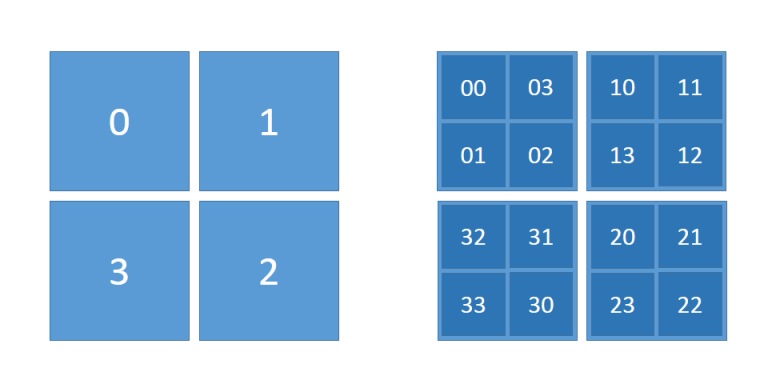
\includegraphics[width=0.65\textwidth]{hilbert}
  \end{center}
\end{frame}

\begin{frame}[t]{More Optimization - Data Layout}
  \begin{itemize}
    \item The order in which edges are presented affects performance.
    \item Hilbert order vs Vertex order.
  \end{itemize}

  \vspace{0.5cm}
  \begin{center}
    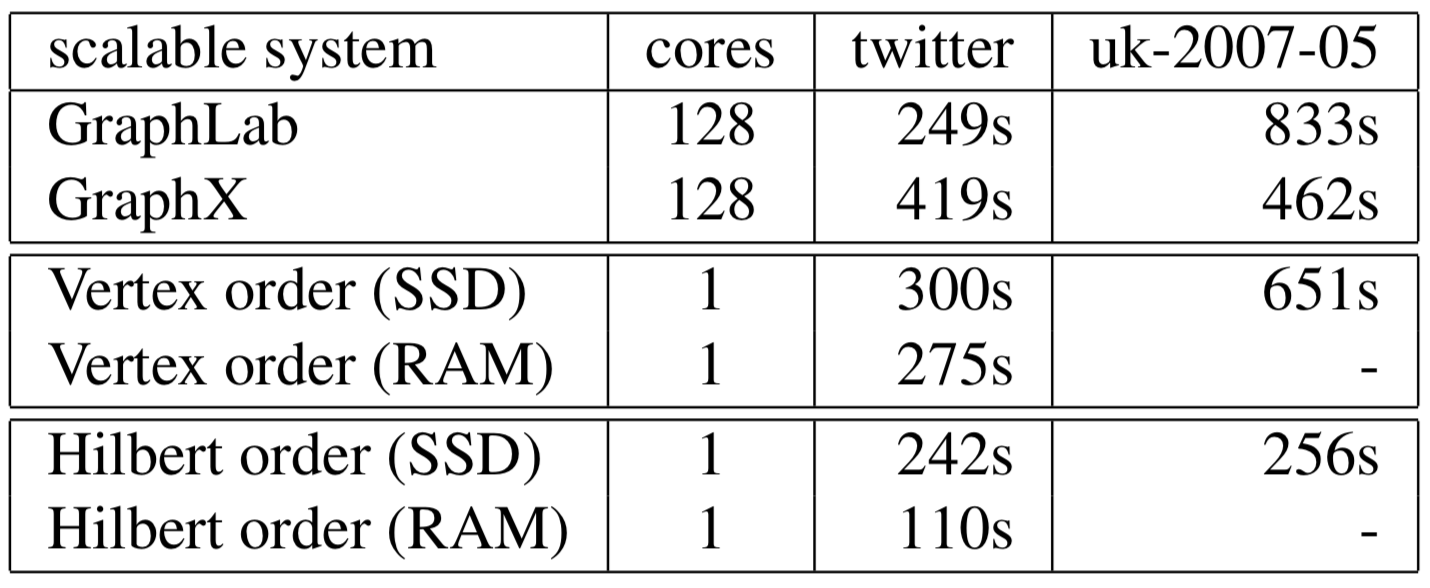
\includegraphics[width=0.75\textwidth]{data-layout}
  \end{center}
\end{frame}

\begin{frame}[t]{Even More Optimization! - Programming Model}
  \begin{itemize}
    \item We are not restricted to "Think like a Vertex" programming model.
    \item Label propagation is sub-optimal, typically $O(n^3 + mn^2)$
    \item Use Weighted Union-Find, $O(m \log{n})$
  \end{itemize}

  \pause

  \vspace{0.5cm}
  \begin{center}
    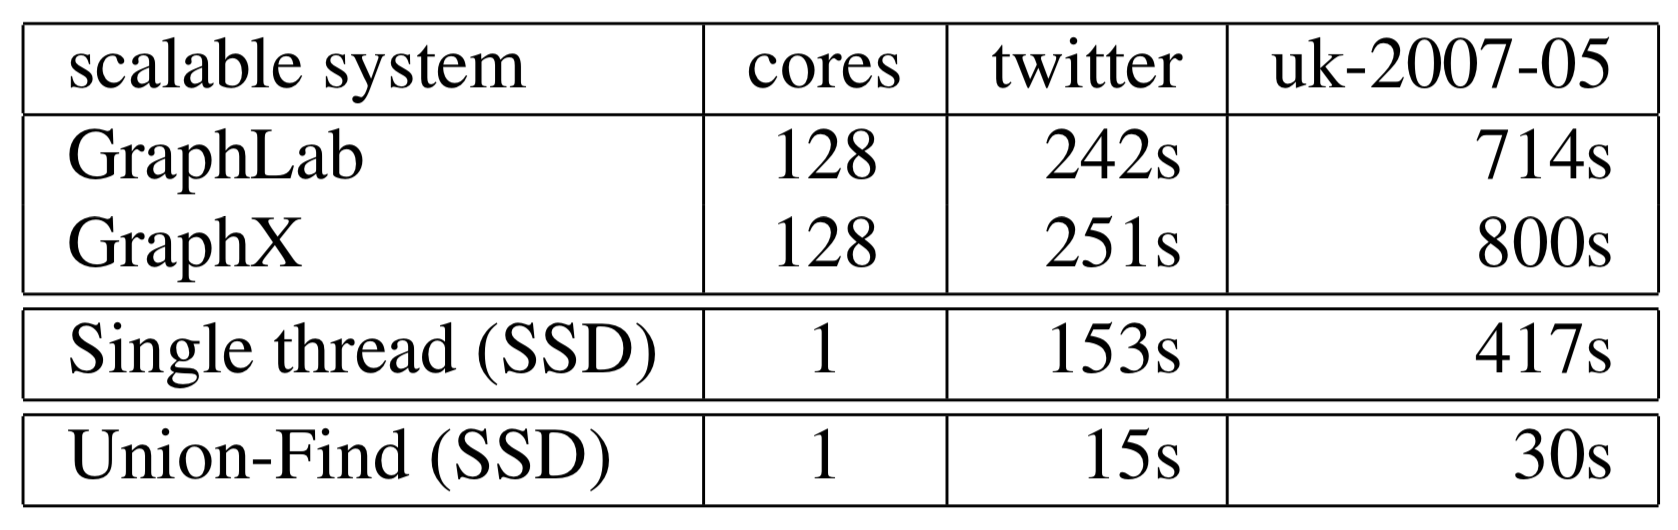
\includegraphics[width=0.75\textwidth]{union-find}
  \end{center}
\end{frame}

\begin{frame}[t]{Applying COST}

  \vspace{0.25cm}

  COST is the point of intersection\footnote{Plots simplified for illustration purposes}

  \begin{center}
    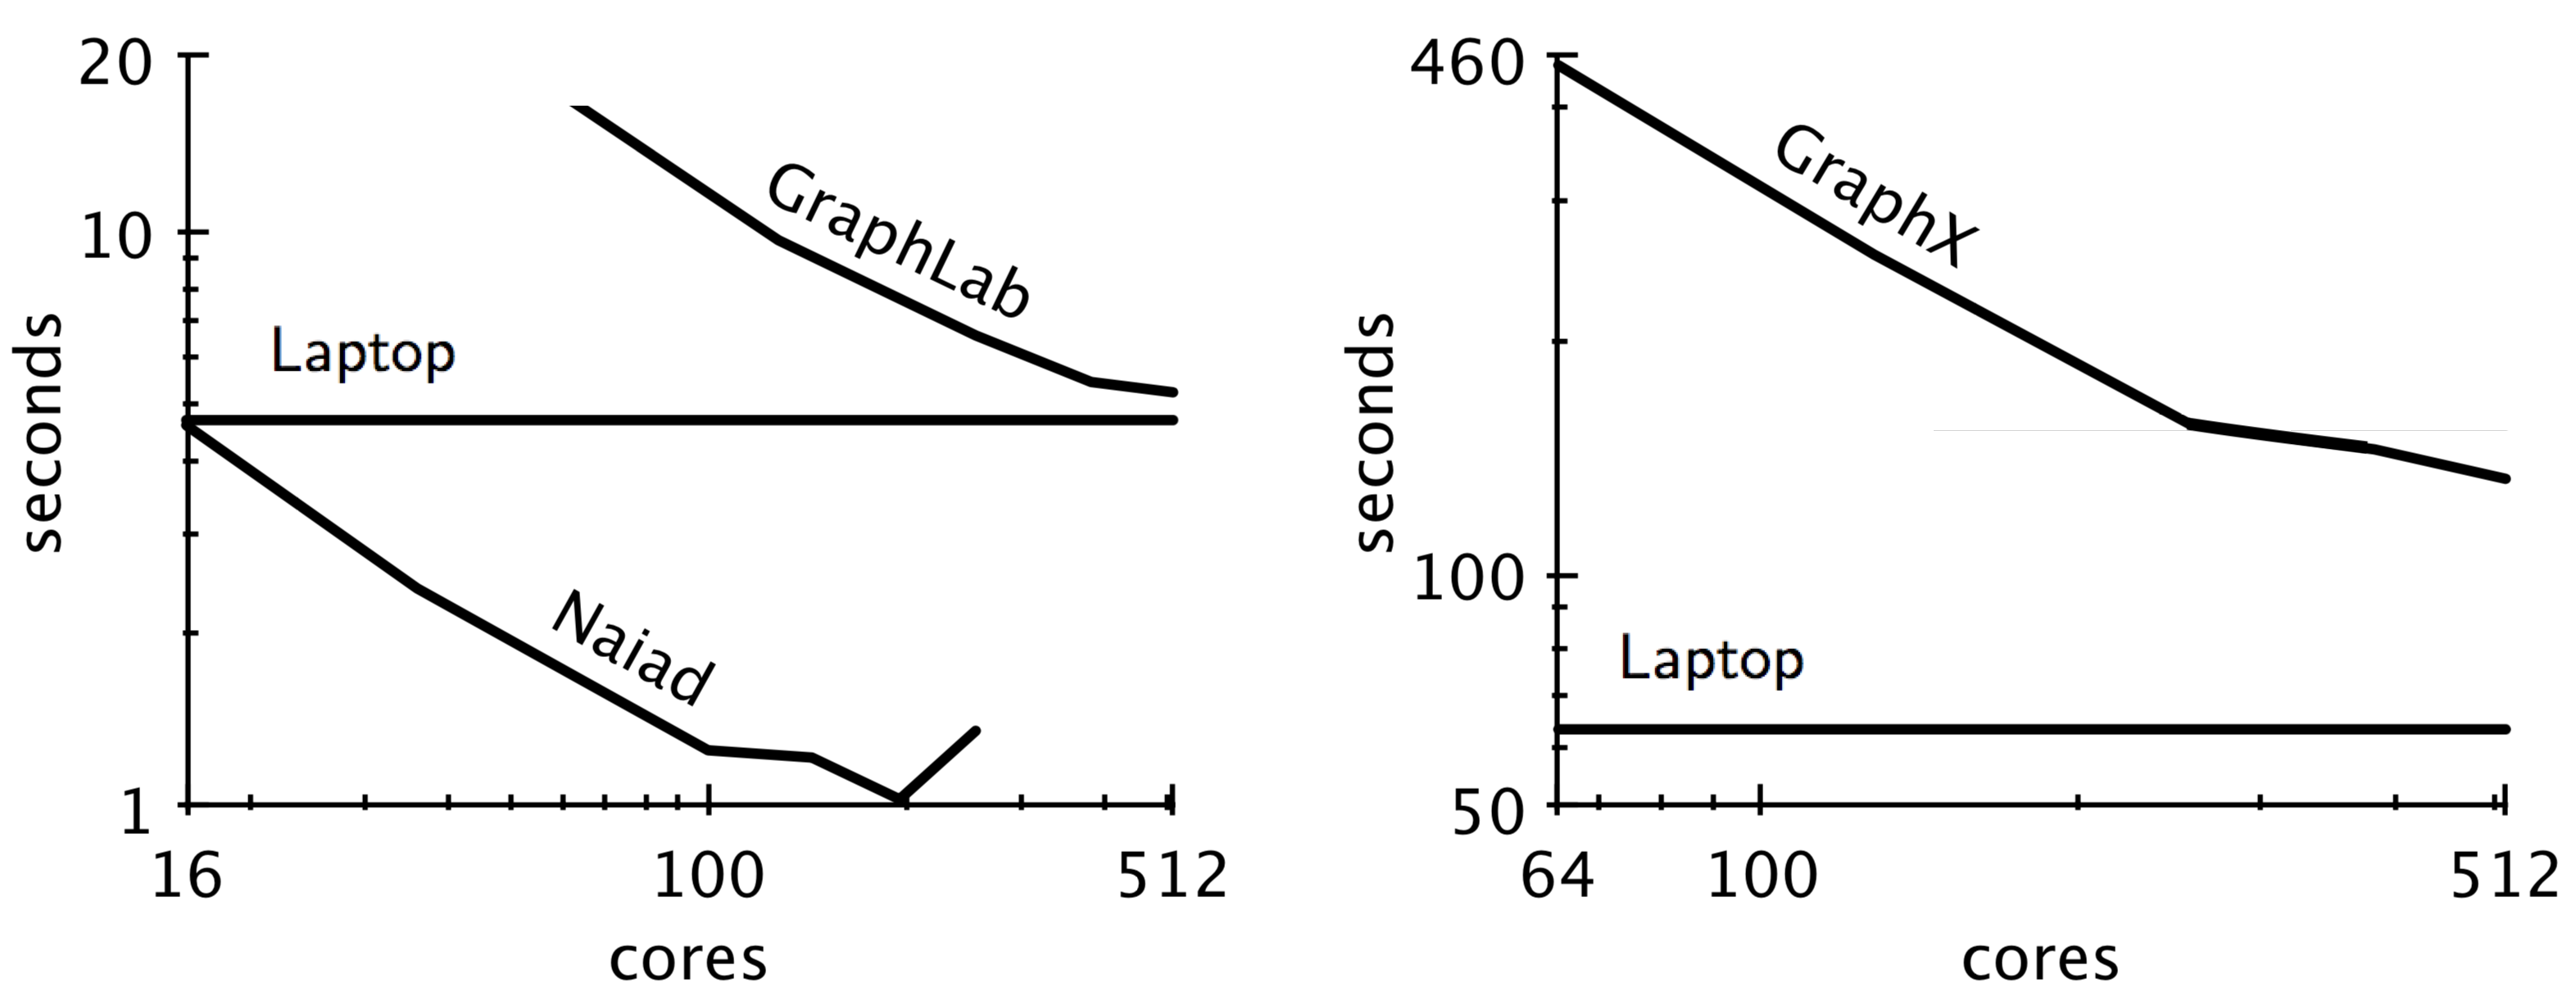
\includegraphics[width=0.95\textwidth]{applying-cost}
  \end{center}

  \pause

  \begin{itemize}
    \item Naiad has a COST of 16 cores for PageRank
    \item GraphX has an unbounded COST (does not intersect)
  \end{itemize}
\end{frame}